 \documentclass{report}
 
\usepackage[utf8]{inputenc} 
\usepackage[T1]{fontenc}      
\usepackage[top=2.0cm, bottom=3cm, left=3.0cm, right=3.0cm]{geometry}
\usepackage{graphicx}
\usepackage{wrapfig}
\usepackage{amsmath,esint }
\usepackage{amssymb}
\graphicspath{{figures/}{../figures}}

\newcommand*\dif{\mathop{}\!\mathrm{d}}
\newcommand*\diver{\mathop{}\!\mathrm{div}}
\newcommand*\grad{\mathop{}\!\mathrm{grad}}

\begin{document}

\section*{Anneaux de Newton}

Une lentille plan-convexe de diamètre $D=OC$, fragment d'une bille de verre d'indice $n$ de rayon $R$ et de contre $C$ est posée sur un miroir plan, le contact ponctuel se trouvant en $O$ (cf figure). On éclaire le dispositif sous incidence normale en lumière monochromatique de longueur d'onde dans le vide $\lambda$.

\begin{figure}[h]
\centering
  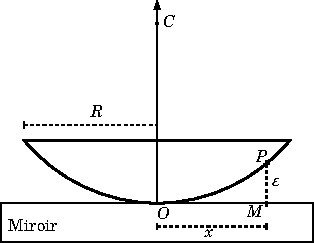
\includegraphics[scale=1.2]{newton.pdf}
\end{figure}

On observe des interférences sur la face sphérique de la lentille et on souhaite comprendre leur origine et en avoir une description détaillée. On supposera dans tout l'exercice que la lentille est mince, c'est-à-dire que $R\ll D$. 

\begin{itemize}

	\item[$\circledcirc$] A l'aide d'un schéma précis, décrire le trajet d'un rayon lumineux traversant la lentille au niveau du point $M$, se réfléchissant au point $P$. Pourquoi voit-on des interférences lumineuses ? On pourra supposer que le rayon n'est pas dévié lorsqu'il sort de la lentille (pourquoi ?).
	
	\item[$\circledcirc$] Expliciter la relation entre l'épaisseur $\varepsilon=PM$ en fonction de $x=OM$ de la couche d'air au point P. 
	
	\item[$\circledcirc$] Montrer que les franges d'interférences sont des cercles concentriques, préciser le rayon de la $n$-ième frange brillante et celui de la $n$-ième frange sombre, en considérant qu'un point central est une frange et en numérotant du centre vers la périphérie.
	
	\item[$\circledcirc$] Décrire ce que l'on observe en lumière blanche.

\end{itemize}

\newpage

\section*{\textit{Correction : Anneaux de Newton}}

\begin{itemize}

	\item[$\circledcirc$] Le rayon arrivant au point $M$ et se réfléchissant au point $P$ interfère avec lui-même lorsqu'il est réfléchi sur le miroir. Les interférences étant visibles au niveau de la face sphérique de la lentille, la différence de marche correspond à deux fois l'épaisseur d'air entre la lentille et le miroir (plus le déphasage à la réflexion).
	
	\item[$\circledcirc$] L'équation de la surface de la lentille s'écrit $(\varepsilon-R)^2+x^2=R^2$. On a alors $\varepsilon=R-\sqrt{R^2-x^2}$ (car on est côté inférieur du cercle), et comme $x<D\ll R$, on a aussi $\varepsilon\simeq x^2/2R$.
	
	\item[$\circledcirc$] Ce sont des cercles concentriques car la lentille à une symétrie par rotation autour de l'axe $OC$ (il suffirait de remplacer $x$ par $r$ ou $\sqrt{x^2+y^2}$). La différence de marche correspond à $\delta=2\varepsilon$. Le déphasage total est donc (avec celui du miroir) :
	\begin{align*}
		\Delta \varphi = \frac{4\pi\varepsilon}{\lambda}+\pi
	\end{align*}
	Pour $x=0$, on a $\Delta \varphi = \pi$, et alors $I=0$ : on a une frange sombre au centre de la lentille. En notant $n$ la $n$-ième frange sombre on a : $\Delta\varphi_n=2n\pi+\pi=\frac{4\pi\varepsilon_n}{\lambda}+\pi$, donc :
	\begin{align*}
		x_n=\sqrt{R\lambda n}
	\end{align*}
	De la même façon, en notant $p$ les franges brillantes, on a :
	$\Delta\varphi_p=2(p+1)\pi=\frac{4\pi\varepsilon_p}{\lambda}+\pi$, donc :
	\begin{align*}
		x_p=\sqrt{R\lambda \left( p+\frac{1}{2}\right) }
	\end{align*}
	
	\item[$\circledcirc$] Le centre est une tâche sombre quelque soit la valeur de $\lambda$. La plus petite des franges brillantes est celle correspondant au $\lambda$ le plus petit, donc c'est la couleur bleu/violet. toutes les autres couleurs s'allument ensuite : on a donc des cercles concentriques irrisés. 

\end{itemize}

\newpage

\section*{Miroir de Fresnel}

Un dispositif interférentiel est constitué de deux miroirs plans $M_1$ et $M_2$ de même surface, faisant entre eux un angle $\varepsilon$. Il est éclairé par une une fente parallèle à l'arête centrale qui sépare les deux miroirs. La lumière émise par cette fente est supposée monochromatique de longueur d'onde $\lambda$. La source $S$ est placée à une distance $d$ de l'arête entre les deux miroirs, dans une position repérée par l'angle $\alpha$ par rapport au plan horizontal. Les angles $\varepsilon$ et $\alpha$ sont supposés très petits. On observe l'image issue des miroirs sur un écran placé à une distance $D$ de l'arête.

\begin{figure}[h]
\centering
  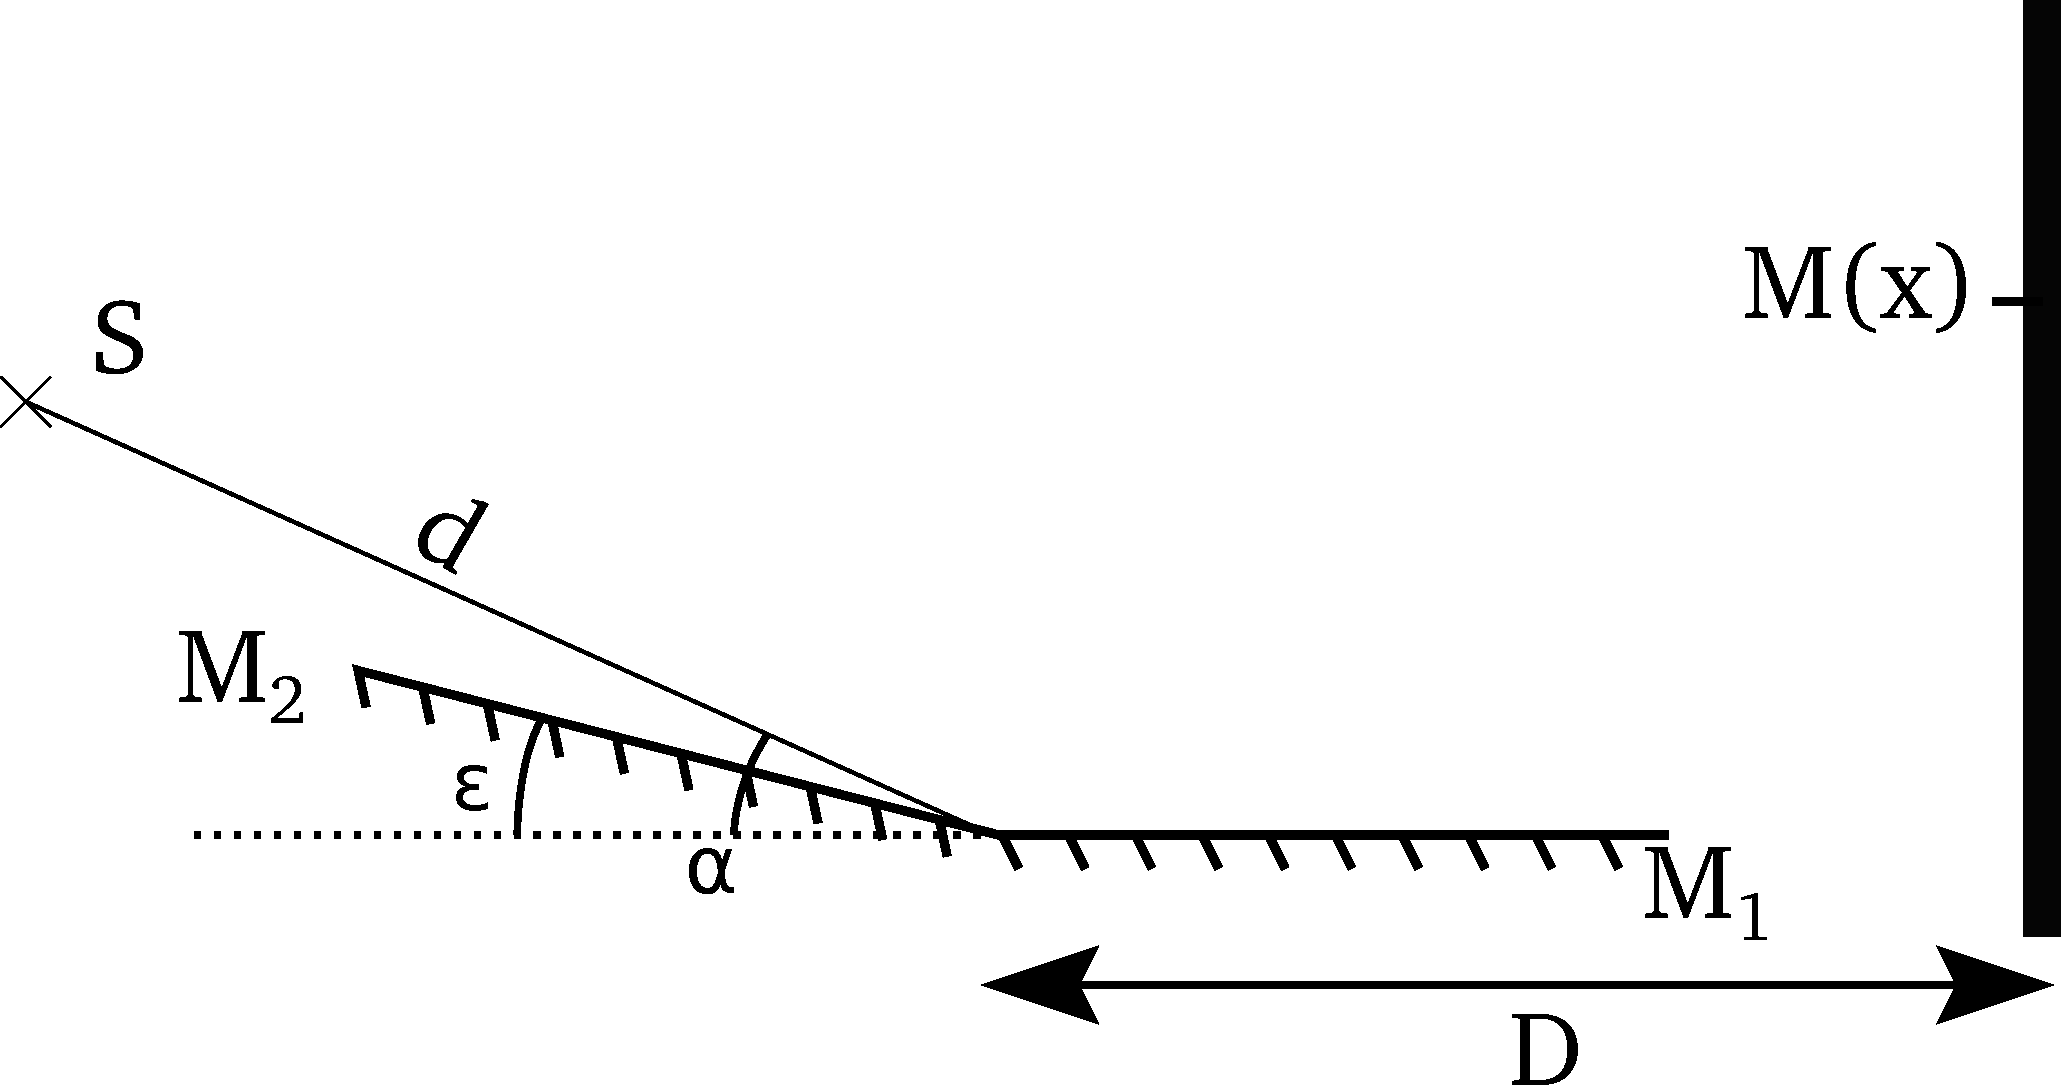
\includegraphics[scale=0.25]{fresnel.pdf}
\end{figure}

\begin{itemize}

	\item[$\divideontimes$] Montrer que l'on peut mettre en évidence deux sources secondaires $S_1$ et $S_2$ correspondant à l'image de la source $S$ dans chaque miroir et donner leur coordonnées. Construire les rayons issus de S arrivant en M.
	
	\item[$\divideontimes$] Montrer que l'on peut considérer ce dispositif comme équivalent à des fentes d'Young. Calculer l'intensité $I$ sur l'écran. En déduire la figure d'interférence.
	
	\item[$\divideontimes$] Déterminer l'interfrange.
	
	\item[$\divideontimes$] Décrire ce que l'on observe en lumière blanche.

\end{itemize}

\newpage

\section*{\textit{Correction - Miroir de Fresnel}}

\begin{itemize}

	\item[$\divideontimes$] $S_1$ est le symétrique de $S$ par rapport au miroir $M_1$ et $S_2$ est le symétrique de $S$ par rapport au miroir $M_2$. 
	
\begin{figure}[h]
\centering
  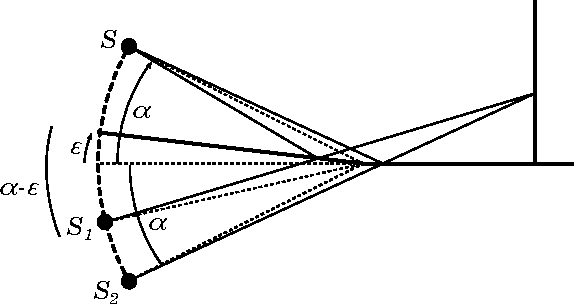
\includegraphics[scale=1.0]{fresnel_cor.pdf}
\end{figure}

Par construction, et en prenant l'origine $O$ sur l'arête, $S_1=(-d\cos\alpha,-d\sin\alpha)$ et $S_2=(-d\cos(\alpha-2\varepsilon),-d\sin((\alpha-2\varepsilon))$
	
	\item[$\divideontimes$] On a donc deux sources secondaires cohérentes. On prend directement $\cos(\alpha)\simeq1$ et $\sin\alpha\simeq\alpha$. Comme $M=(x+d,y)$, on peut calculer la différence de marche :
	\begin{align*}
		\delta &= S_1M-S_2M \\
		&=\sqrt{•}
	\end{align*}
	
	\item[$\divideontimes$] Déterminer l'interfrange.
	
	\item[$\divideontimes$] Décrire ce que l'on observe en lumière blanche.

\end{itemize}

\newpage

\section*{Fentes d'Young élargies}

On s'intéresse à un dispositif de fente d'young comme représenté sur le schéma ci-dessous. Une source lumineuse, ponctuelle (d'intensité $I$), monochromatique (longueur d'onde $\lambda$), est située à une distance $Y$ de l'origine du plan $(O_1,X,Y)$. Celui-ci est placé à une distance $d$ d'un plan opaque sur lequel deux petits trous sont distants de $a$ suivant l'axe $Y$, symétriques par rapport à l'axe $O_1O_2$.A une distance $D$ de ce plan, on observe l'intensité lumineuse sur un écran, repéré par le plan $(O_2,x,y)$. On supposera que $d$ et $D$ sont gr	ands devant les autres distances.

\begin{figure}[h]
\centering
  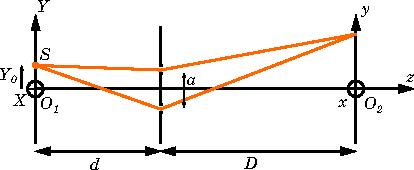
\includegraphics[scale=1.0]{young1.pdf}
\end{figure}

\begin{itemize}

	\item[$\gtrdot$] Exprimer la différence de marche $\delta$ pour deux rayons lumineux arrivant au point $M$ sur l'écran. En déduire l'intensité $I(x,y)$.
	
	\item[$\gtrdot$] Quelle est l'allure des franges d'interférences ? Comment évoluent celles-ci évoluent en fonction de $Y$ ?

\end{itemize}

On suppose désormais que la source lumineuse n'est plus ponctuelle, mais a une largeur $b$ (uniquement suivant $O_1Y$) et est placée symétriquement par rapport à l'axe $O_1O_2$. La puissance de la source est homogène, c'est-à-dire que tous ses points emettent une intensité par unité de longueur identique.

\begin{figure}[h]
\centering
  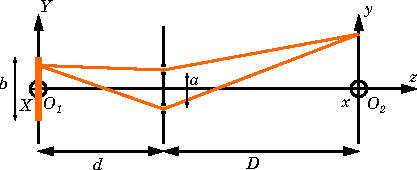
\includegraphics[scale=1.0]{young2.pdf}
\end{figure}

\begin{itemize}

	\item[$\gtrdot$] Quelle est l'intensité $dI(x,y)$ sur l'écran dû à un point de la source de largeur $dy$ situé à une distance $Y$ ?
	
	\item[$\gtrdot$] En déduire l'intensité totale $I(x,y)$ sur l'écran dûe à la source dans toute sa largeur $b$. Pourquoi peut-on simplement sommer la contribution de tous les points de la source ?
	
	\item[$\gtrdot$] Exprimer le constraste $C$.

\end{itemize}

\end{document}